\documentclass[../classical_mechanics.tex]{subfiles}

\begin{document}

    % TODO: add an interlude on 3D spherical and cylindrical coordinates

    \section{Moments}
        \paragraph{}
        When dealing with problems involving rotation, we have mechanical quantities which are analogous to ones used to solve linear problems.
        We have seen a few of these before: angular velocity $\omega=v_\theta/r$, angular acceleration $\alpha=a_\theta/r$ (for circular motion), and moment of inertia $I=mr^2$.
        As we can see, the definitions of these quantities all involve the analogous linear quantity and the distance from the origin $r$.
        Quantities that involve the \textit{product} of a linear quantity with the radius are called \textbf{moments}.
        Moments we have seen already are the center of mass, which is the first moment of mass (sum of $mr$) normalised by the total mass, and the moment of inertia, which is the second moment of mass (mass multiplied by $r^2$)
        In this chapter we will introduce two more moments: torque --- the moment of force --- and angular momentum --- the moment of momentum.
        When vector quantities like force and momentum are involved, moments are defined using the cross product.
        \begin{definition}
            \textbf{Angular Momentum} is defined as the first moment of momentum.
            \begin{equation}
                \vec{L}=\vec{r}\times\vec{p}=m\vec{r}\times\vec{v}.
            \end{equation}
        \end{definition}
        Note that because the cross product is antisymmetric, the order of $\vec{r}$ and $\vec{p}$ matters!
        The motivation for introducing angular momentum will become clear in the next section. 

    \section{Central Forces}
        \paragraph{}
        We will now examine a very special type of force.
        These forces have many useful properties which make solving problems involving them a lot simpler.
        \begin{definition}
            A \textbf{central force} is a force which acts along the radial direction and only depends on the radial distance $r$.
            Central forces thus have the form
            \begin{equation}
                \vec{F}=F(r)\uvec{r}.
            \end{equation}
            If $F(r)<0$, the force is attractive, and if $F(r)>0$, the force is repulsive.
        \end{definition}
        We have seen one example of a central force already, the universal law of gravitation.
        Another example is Coulomb's law.

        \paragraph{}
        Motion under a central force obeys the following rules:
        \begin{itemize}
            \item The motion is confined to a plane.
            \item The angular momentum is conserved ($\dv{\vec{L}}{t}=0$).
            \item The position vector sweeps out equal area in equal time.
        \end{itemize}
        
        \paragraph{}
        Let's prove that angular momentum is conserved under the influence of a central force.
        Looking at the derivative, we get
        \begin{align}
            \dv{\vec{L}}{t}&=\dv{}{t}(\vec{r}\times\vec{p})\\
            &=\dv{\vec{r}}{t}\times\vec{p}+\vec{r}\times\dv{\vec{p}}{t}\\
            &=\vec{v}\times m\vec{v}+\vec{r}\times F(R)\uvec{R}\\
            &=0.
        \end{align}
        Therefore, $\vec{L}$ is constant over time, it is conserved.

        \paragraph{}
        By definition, $\vec{L}$ is perpendicular to $\vec{r}$.
        We can also see this by taking the dot product of $\vec{L}$ with the position vector:
        \begin{equation}
            \vec{r}\cdot\vec{L}=\vec{r}\cdot(\vec{r}\times\vec{p})=\vec{p}\cdot(\vec{r}\times\vec{r})=0.
        \end{equation}
        Since $\vec{L}$ is constant, this implies that $\vec{r}$ is confined to the plane perpendicular to $\vec{L}$.
        
        \paragraph{}
        Because of this, it is convenient to use cylindrical coordinates with the plane $z=0$ as the plane of motion.
        Using equation~\ref{} (note that $\dot{z}=0$) and the cross products between unit vectors, we get
        % TODO: add reference to velocity in cylindrical coordinates here
        \begin{align}
            \vec{L}&=m\vec{r}\times\vec{v}\\
            &=mR\uvec{R}\times(\dot{R}\uvec{R}+R\dot{\theta}\uvec{\theta})\\
            &=mR^2\dot{\theta}\khat\label{eq:angular-momentum-theta-dot}\\
            &=mh\khat.
        \end{align}
        In the last line we have defined $h=R^2\dot{\theta}$.
        This is the \textbf{specific angular momentum} (angular momentum normalised by mass), and is useful in some problems.

        Finally, we will prove the last fact about motion under central forces, the law of equal areas, which is a more general version of Kepler's second law of planetary motion.
        Consider an object on a curved path at two points separated by a small time interval $\dd{t}$.
        \begin{figure}[H]
            \centering
            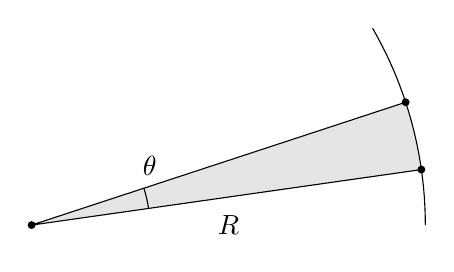
\begin{tikzpicture}[scale=5]
                \fill[fill=black!10,rotate=8] (0,0) -- (1,0) arc [radius=1, start angle=0, end angle=10.1] -- cycle;
                \draw[rotate=8] (0.3,0) arc [radius=0.3, start angle=0, end angle=10.1];
                \draw (1,0) arc [radius=1, start angle=0, end angle=30];
                \draw (0,0) -- (0.95,0.312) (0.99,0.141) -- (0,0);
                \fill (0.95,0.312) circle [radius=0.01];
                \fill (0.99,0.141) circle [radius=0.01];
                \fill (0,0) circle [radius=0.01];
                \node at (0.3,0.15) {$\dd{\theta}$};
                \node at (0.5,0) {$R$};
            \end{tikzpicture}
        \end{figure}
        The shaded arc is approximately a triangle, so the area get closer and closer to $A=\frac{1}{2}R^2\dd{\theta}$ as $\dd{t}\to0$.
        Therefore, we have
        \begin{equation}
            \dv{A}{t}=\frac{1}{2}R^2\dv{\theta}{t}=\frac{1}{2}h=\text{const}.
        \end{equation}
        So the rate of area swept out over time is constant.

        \paragraph{}
        What does motion under a central force look like?
        By Newton's second law, we know that
        \begin{equation}\label{eq:central-force-eom}
            a_R=\ddot{R}-R\dot{\theta}^2=\frac{F(R)}{m}.
        \end{equation}
        Substituting in the specific angular momentum, we get
        \begin{equation}
            \ddot{R}-\frac{h^2}{R^3}=\frac{F(R)}{m}.
        \end{equation}
        This is the differential equation we need to solve for any central force problem.
        \begin{example}
            Prove Kepler's third law: the square of a planet's orbital period is proportional to the cube of the semi-major axis of its orbit.

            \paragraph{}
            Planets move according to the universal law of gravitation, which is
            \begin{equation}
                \vec{F}=-\frac{GMm}{R^2}\uvec{R}.
            \end{equation}
            We will make an approximation and assume that the sun is fixed at the origin and the planets orbit in circular orbits.
            In reality, the a given planet and the sun orbit their common centre of mass in elliptical paths, but the difference is very small making this approximation makes the problem much simpler.
            Since $R=\text{const}$, then $\dot{R}=\ddot{R}=0$.
            So $a_R=-R\dot{\theta}^2$.
            Since angular momentum $L=mR^2\dot{\theta}$ is conserved, $\dot{\theta}=\omega$ is a constant.
            Thus the equation of motion \ref{eq:central-force-eom} becomes
            \begin{align}
                -\frac{GMm}{R^2}&=-mR\omega^2\\
                GM&=R^3\omega^2.
            \end{align}
            The period of the orbit is equal to the displacement divided by the speed, in this case $T=\frac{2\pi}{\omega}$, so rearranging for $R^3$ we get
            \begin{equation}
                R^3=\frac{GM}{4\pi^2}T^2.
            \end{equation}
        \end{example}
        \begin{example}
            Consider a central force of the form $\vec{F}=-\frac{mk^2}{r^3}\uvec{r}$.
            If a particle under the influence of this force starts at a distance $r=r_0$ from the origin with no radial speed ($v_{r,0}=0$), what will its motion look like for different values of $k$?

            \paragraph{}
            Substituting in the force into equation~\ref{eq:central-force-eom}, we get
            \begin{gather}
                \ddot{r}-\frac{h}{r^3}=-\frac{k^2}{r^3}\\
                \ddot{r}+\frac{k^2-h^2}{r^3}=0.
            \end{gather}
            For $k^2=h^2$, we get $\ddot{r}=0$, which can be integrated twice to give $r=r_0+v_{r,0}t$.
            Since $v_{r,0}=0$, we have $r=r_0$ which is circular motion.
            The angular speed is given by equation~\ref{eq:angular-momentum-theta-dot}, $\omega=\frac{L}{mr_0^2}=\frac{mvr_0}{mr_0^2}=\frac{v}{r_0}$.
            This is just our familiar result from uniform circular motion, which makes sense because if we plug $k^2=h^2$ into the form of the force above, we get
            \begin{equation}
                \vec{F}=-\frac{mr^4\omega^2}{r^3}\uvec{r}=-mr\omega^2\uvec{r},
            \end{equation}
            which is just the formula for centripetal force.

            \paragraph{}
            What about the cases where $k^2\neq h^2$?
            Unfortunately, the differential equation is not solvable analytically for any other case.
            Luckily, there is another way to solve it!
            What we have to do is parameterise the orbit in terms of the angular displacement $\theta$ instead of $t$ by making use of the relation $h=r^2\dot{\theta}$.
            We will also make the substition $u=1/r$, which is a very useful substition when solving problems with central forces of the form $F(r)=\frac{\alpha}{r^n}$.
            Therefore, the aim is to replace all time derivatives of $r$ with derivatives of $u$ with respect to $\theta$.
            Using the chain rule, we get
            \begin{align}
                \dot{r}&=\dv{r}{u}\dot{u}=\dv{r}{u}\dv{u}{\theta}\dot{\theta}\\
                &=-r^2\dot{\theta}\dv{u}{\theta}\\
                &=-h\dv{u}{\theta}.
            \end{align}
            For $\ddot{r}$, we get
            \begin{align}
                \ddot{r}&=\dv{}{t}\left(-h\dv{u}{\theta}\right)=-h\dv[2]{u}{\theta}\dot{\theta}\\
                &=-\frac{h^2}{r^2}\dv[2]{u}{\theta}\\
                &=-h^2u^2\dv[2]{u}{\theta}.
            \end{align}
            Now, the equation of motion becomes
            \begin{gather}
                -h^2u^2\dv[2]{u}{\theta}+(k^2-h^2)u^3=0\\
                \dv[2]{u}{\theta}-\frac{k^2-h^2}{h^2}u=0.
            \end{gather}

            \paragraph{}
            Letting $\beta^2=\abs{\frac{k^2-h^2}{h^2}}$, if $k^2>h^2$ then the differential equation becomes
            \begin{equation}
                \dv[2]{u}{\theta}-\beta^2 u=0.
            \end{equation}
            The general solution is $u=Ae^{\beta\theta}+Be^{-\beta\theta}$.

            \paragraph{}
            For the opposite case $k^2<h^2$, the negative sign gets cancelled out and we get
            \begin{equation}
                \dv[2]{u}{\theta}+\beta^2 u=0.
            \end{equation}
            This has the general solution $u=A\cos(\beta\theta)+B\sin(\beta\theta)$.

            % TODO: complete this example.
        \end{example}

    \section{Torque}
        \paragraph{}
        Torque is defined as the \textbf{moment} of force, that is, the product of the distance from a reference point and the force.
        % TODO: include a proper discussion of pivot points and what torque does
        In terms of vectors, this is given by the cross product
        \begin{equation}
            \vec{N}=\vec{r}\times\vec{F}.
        \end{equation}
        The magnitude of $\vec{N}$ is given by
        \begin{align}
            N&=\abs{\vec{r}}\abs{\vec{F}}\sin\theta\\
            &=rF_\text{tan}.
        \end{align}
        % TODO: include diagram for this
        This formula tells us that for a fixed radius, the torque has maximum magnitude when $\theta=\pm\frac{\pi}{2}$ i.e. the force acts \textit{perpendicular} to the radius.
        It also tells us that if the force acts along the same line as the radius ($\theta=0$ or $\theta=\pi$), then the torque is equal to 0.
        Since torque is defined as a moment like angular momentum, its value is relative to an arbitrary reference point.
        Changing the reference point will change the value of the torque.
        For a fixed reference point, if the same force is applied further away from the centre, the torque will be greater.
        
        \paragraph{}
        Let's look at how changing the reference point changes the angular momentum and the torque.
        Consider the following diagram.
        \begin{figure}[H]
            \centering
            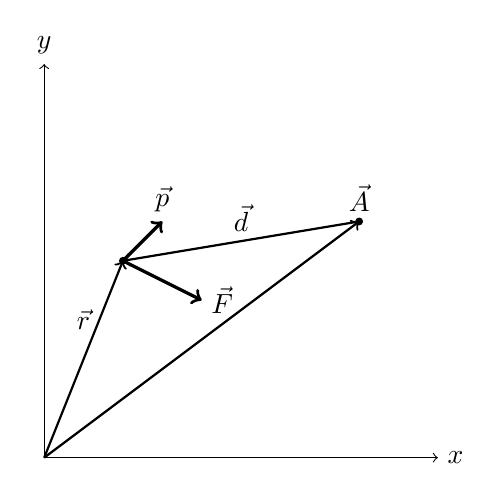
\begin{tikzpicture}[scale=5]
                \draw[<->] (0,1) |- (1,0);
                \node[above] at (0,1) {$y$};
                \node[right] at (1,0) {$x$};

                \draw[->,thick] (0,0) -- (0.2,0.5);
                \fill (0.2,0.5) circle [radius=0.01];
                \node[above] at (0.1,0.3) {$\vec{r}$};
                \draw[<->,very thick] (0.3,0.6) -- (0.2,0.5) -- (0.4,0.4);
                \node[above] at (0.3,0.6) {$\vec{p}$};
                \node[right] at (0.4,0.4) {$\vec{F}$};

                \draw[->,thick] (0,0) -- (0.8,0.6);
                \fill (0.8,0.6) circle [radius=0.01];
                \node[above] at (0.8,0.6) {$\vec{A}$};
                
                \draw[->,thick] (0.8,0.6) -- (0.2,0.5);
                \node[above] at (0.5,0.55) {$\vec{d}$};
            \end{tikzpicture}
        \end{figure}
        The angular momentum and torque relative to the origin are $\vec{L}=\vec{r}\times\vec{p}$ and $\vec{N}=\vec{r}\times\vec{F}$ like before, but what are the angular momentum and torque relative to the point $\vec{A}$?
        The radius vector or lever arm is now the vector $\vec{d}$ between the points $\vec{A}$ and $\vec{r}$, i.e.
        \begin{align}
            \vec{L}_{\vec{A}}&=\vec{d}\times\vec{p}\\
            &=(\vec{r}-\vec{A})\times\vec{p}\\
            \vec{N}_{\vec{A}}&=\vec{d}\times\vec{F}\\
            &=(\vec{r}-\vec{A})\times\vec{F}.
        \end{align}
        \begin{example}
            Consider a \qty{2}{\kilogram} particle at $y=\qty{3}{\meter}$ moving to the right with velocity $\vec{v}=\qty{5}{\meter\per\second}\ihat$.
            What is its angular momentum relative to the origin and relative to the point $\vec{A}=\qty{3}{\meter}\jhat$.
            \begin{figure}[H]
                \centering
                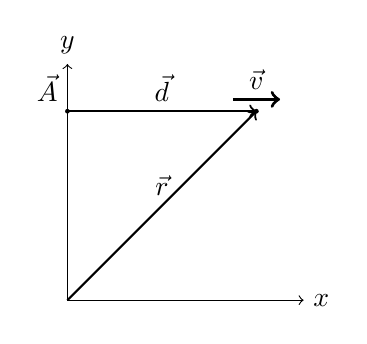
\begin{tikzpicture}[scale=3]
                    \draw[<->] (0,1) |- (1,0);
                    \node[above] at (0,1) {$y$};
                    \node[right] at (1,0) {$x$};

                    \fill (0,0.8) circle [radius=0.01];
                    \node[above left] at (0,0.8) {$\vec{A}$};

                    \fill (0.8,0.8) circle [radius=0.01];
                    \draw[->,very thick] (0.7,0.85) -- (0.9,0.85);
                    \node[above] at (0.8,0.85) {$\vec{v}$};

                    \draw[->,thick] (0,0.8) -- (0.8,0.8);
                    \node[above] at (0.4,0.8) {$\vec{d}$};
                    \draw[->,thick] (0,0) -- (0.8,0.8);
                    \node[above] at (0.4,0.4) {$\vec{r}$};
                \end{tikzpicture}
            \end{figure}
            The position vector is $\vec{r}=x\ihat+\qty{3}{\meter}\jhat$ and the radius vector relative to $\vec{A}$ is $\vec{d}=x\ihat$.
            The momentum vector is $\vec{p}=mv_x\ihat=\qty{10}{\kilogram\meter\per\second}$, so the angular momentum relative to the origin is
            \begin{align}
                \vec{L}&=\vec{r}\times\vec{p}=\begin{vmatrix}
                    \ihat & \jhat & \khat \\
                    x & 3 & 0 \\
                    10 & 0 & 0
                \end{vmatrix}\\
                &=-\qty{30}{\kilogram\meter\squared\per\second}\khat,
            \end{align}
            at the angular momentum relative to $\vec{A}$ is
            \begin{align}
                \vec{L}_{\vec{A}}&=\vec{d}\times\vec{p}=\begin{vmatrix}
                    \ihat & \jhat & \khat \\
                    x & 0 & 0 \\
                    10 & 0 & 0
                \end{vmatrix}\\
                &=0.
            \end{align}
            This makes sense because relative to $\vec{A}$ the motion is radial so there is no lever arm.
        \end{example}
        \begin{example}
            Let's now look at a familiar example, uniform circular motion.
            First, what is the angular momentum relative to the origin for a particle travelling with angular speed $\omega$?

            \paragraph{}
            Working in polar coordinates, the radius vector is $\vec{r}=r\uvec{r}$ and the velocity vector is $\vec{v}=r\omega\uvec{\theta}$.
            Then the angular momentum is $\vec{L}=r\uvec{r}\times mr\omega\uvec{\theta}=mr^2\omega\khat$.
            This is a constant, which we know to be the case since the centripetal force is a central force.

            \paragraph{}
            Now, suppose the particle is moving around a circle at $y=h$.
            What is the angular momentum relative to the origin?
            % TODO: include diagram for this

            \paragraph{}
            The position vector is now given by $\vec{r}=r\uvec{r}+h\khat$, so the angular momentum becomes
            \begin{align}
                \vec{L}&=m\begin{vmatrix}
                    \uvec{r} & \uvec{\theta} & \khat \\
                    r & 0 & h \\
                    0 & r\omega & 0
                \end{vmatrix}\\
                &=-mhr\omega\uvec{r}+mr^2\omega\khat.
            \end{align}
            The unit vector $\uvec{r}$ changes over time, so $\vec{L}$ is not constant (its magnitude is constant but its direction changes).
            This is because the centripetal force is no longer central relative to the origin.
        \end{example}

        \paragraph{}
        Torque is measured in $\unit{\newton\meter}$.
        This is dimensionally equivalent to Joules, but this does not mean that torque is a kind of energy.
        Energy is a scalar quantity, whereas torque is a vector, so they are really different things.

        \paragraph{}
        In linear dynamics, we have Newton's second law which states $\vec{F}=\dot{\vec{p}}$.
        We will now show that there is a rotational equivalent of Newton II that relates torque to angular momentum.
        Using the product rule to differentiate $\vec{L}$, we find
        \begin{align}
            \dv{\vec{L}}{t}&=\dv{}{t}(\vec{r}\times\vec{p})\\
            &=(\dot{\vec{r}}\times\vec{p})+(\vec{r}\times\dot{\vec{p}})\\
            &=\left(\frac{1}{m}\vec{p}\times\vec{p}\right)+(\vec{r}\times\vec{F})\\
            &=\vec{r}\times\vec{F}=\vec{N}.
        \end{align}
        This is the same calculation we did earlier for central forces.
        We now have a shortcut to prove that angular momentum is conserved under the influence of a central force.
        % TODO: add equation references
        Since central forces are always parallel to the radius vector, the torque is zero.
        \begin{equation}
            \vec{N}=\vec{r}\times F(r)\uvec{r}=0.
        \end{equation}
        Then using the angular equivalent of Newton II, $\dot{\vec{L}}=\vec{N}=0$.
        So central forces exert no torque and therefore angular momentum is conserved.

        \paragraph{}
        Using Newton's second law on the equation above, we can write the equation for torque above as
        \begin{equation}
            \tau=\sum_i\tau_i=\sum_im_ir_ia_i=\sum_im_ir_i^2\alpha=I\alpha.
        \end{equation}
        % TODO: include vector version of this
        This works because for a rigid body, the angular acceleration is the same for all parts of the body, just like angular velocity.
        We can see from this we have an perfect angular analogue of Newton's second law for torques.
        \begin{example}
            Consider two connected masses on a massless pulley with $m_1>m_2$.
            Suppose the system starts from rest and assume the string is massless, inextensible, and lies vertically.
            Find an expression for the magnitude of acceleration of the masses.
            % TODO: include diagram for this
            To do this, we have to analyse the forces acting on the blocks and also the torques acting on the pulley.
            % TODO: complete this example
        \end{example}

    \section{Static Equilibrium}
        \paragraph{}
        In the net force and the net torque on a rigid body are both 0, then it is in \textbf{static equilibrium}.
        % TODO: include discussion of whether objects can be rotating in static equilibrium
        % TODO: include discussion about how static equilibrium implies net torque is zero in ALL inertial reference frames
        \begin{eqnarray}
            \sum_i\vec{F}_i=0\quad\text{and}\quad\sum_i\vec{\tau}_i=0.
        \end{eqnarray}
        Note that we are free to choose any point as the origin to make finding the net torqe easier.
        \begin{example}
            Consider a beam of mass 10kg and length 4m.
            It sits on a fulcrum placed 1m from one end of the beam, and is supported from the other end by a string.
            Find the tension in the string and the force of the beam on the fulcrum.
            % TODO: complete this example
        \end{example}
        \begin{example}
            A ladder weighing 10kg rests on a smooth wall.
            Find the the static friction force between the floor and the ladder.
            % TODO: complete this example
        \end{example}
        \begin{example}
            Consider a sign hanging from a bar attached to a wall supported by a string.
            Find the force between the bar and the wall.
            % TODO: complete this example
        \end{example}

\end{document}
